\subsubsection{损失函数意义下的最优性}\label{sec:8.3.5}\index{SI0244@决策论}\index{SI0492@决策论}
可以像\autoref{sec:7.3.4}那样，通过决策论分析来比较假设检验，而不只通过功效函数比较. 为作这种分析，必须为假设检验问题指定行动空间和损失函数.

假设检验问题只允许两种行动：“接受 $H_0$”或“拒绝 $H_0$”，可分别记为 $a_0,a_1$. 行动空间是两点集合 $\mathscr A=\{a_0,a_1\}$.\index{SI0004@行动空间}\semanticindexanchor{4:355} 决策规则 $\delta(\boldsymbol x)$（一个假设检验）是样本空间 $\mathscr X$ 上只取 $a_0,a_1$ 两个值的函数. 集合 $\{\boldsymbol x:\delta(\boldsymbol x)=a_0\}$ 是接受域，$\{\boldsymbol x:\delta(\boldsymbol x)=a_1\}$ 是拒绝域，正如\autoref{def:8.1.3}.

假设检验问题的损失函数应反映：若 $\theta\in\Theta_0$ 却选择 $a_1$，或 $\theta\in\Theta_0^c$ 却选择 $a_0$，就犯了错误；另外两种可能情形则作出了正确决定. 由于只有两种可能行动，损失函数 $L(\theta,a)$ 只含两部分. $L(\theta,a_0)$ 是决定接受 $H_0$ 时，在不同 $\theta$ 值下产生的损失；$L(\theta,a_1)$ 则是决定拒绝 $H_0$ 时的损失.

检验问题中最简单的损失称为 $0$–$1$ 损失（$0$–$1$ loss），定义为
$$L(\theta,a_0)=\begin{cases}0,&\theta\in\Theta_0,\\1,&\theta\in\Theta_0^c,\end{cases}
\qquad L(\theta,a_1)=\begin{cases}1,&\theta\in\Theta_0,\\0,&\theta\in\Theta_0^c.\end{cases}$$
采用 $0$–$1$ 损失时，正确决定的损失为 $0$，错误决定的损失为 $1$. 这是两类错误后果相同的一种特别简单的情形. 稍微更现实的损失，是为两类错误赋予不同代价的广义 $0$–$1$ 损失（generalized $0$–$1$ loss）：
\begin{equation}\label{eq:8.3.11}\index{SI0655@广义零一}\index{SI0656@假设检验}\index{SI0663@零一}
L(\theta,a_0)=\begin{cases}0,&\theta\in\Theta_0,\\c_{\mathrm{II}},&\theta\in\Theta_0^c,\end{cases}
\qquad L(\theta,a_1)=\begin{cases}c_{\mathrm I},&\theta\in\Theta_0,\\0,&\theta\in\Theta_0^c.\end{cases}
\end{equation}
这里 $c_{\mathrm I}$ 是第一类错误、即错误拒绝 $H_0$ 的代价，$c_{\mathrm{II}}$ 是第二类错误、即错误接受 $H_0$ 的代价. （实际上，比较检验时真正重要的只是比值 $c_{\mathrm{II}}/c_{\mathrm I}$，不是两个单独的值. 若 $c_{\mathrm I}=c_{\mathrm{II}}$，实质上就是 $0$–$1$ 损失.）

决策论分析用风险函数（期望损失）评价假设检验程序. 检验的风险函数与功效函数密切相关，如下列分析所示.

设 $\beta(\theta)$ 是基于决策规则 $\delta$ 的检验的功效函数，即若用 $R=\{\boldsymbol x:\delta(\boldsymbol x)=a_1\}$ 表示拒绝域，则
$$\beta(\theta)=P_\theta(\boldsymbol X\in R)=P_\theta(\delta(\boldsymbol X)=a_1).$$
\sourcepageanchor{356}

\begin{figure}[htbp]\centering
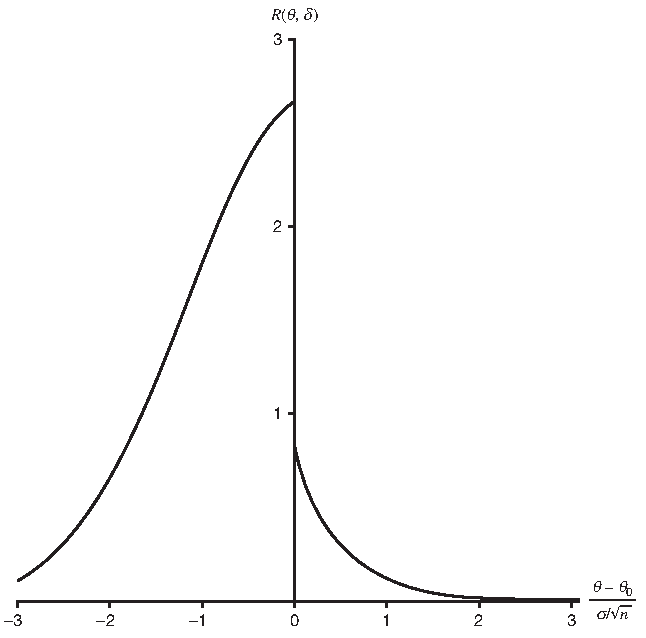
\includegraphics[width=.8\textwidth]{assets/chapter8/fig8-3-4.pdf}
\caption{\autoref{ex:8.3.31}中检验的风险函数，其中 $z=\sqrt n(\theta-\theta_0)/\sigma$.}\label{fig:8.3.4}
\end{figure}

与\eqref{eq:8.3.11}相应、特别是与 $0$–$1$ 损失相应的风险函数非常简单. 对任意 $\theta\in\Theta$，$L(\theta,a)$ 只取两个值：若 $\theta\in\Theta_0$，为 $0$ 和 $c_{\mathrm I}$；若 $\theta\in\Theta_0^c$，为 $0$ 和 $c_{\mathrm{II}}$. 所以风险为
\begin{equation}\label{eq:8.3.12}\index{SI0505@与风险的关系}
\begin{aligned}
R(\theta,\delta)&=0P_\theta(\delta(\boldsymbol X)=a_0)+c_{\mathrm I}P_\theta(\delta(\boldsymbol X)=a_1)\\
&=c_{\mathrm I}\beta(\theta),&&\theta\in\Theta_0;\\
R(\theta,\delta)&=c_{\mathrm{II}}P_\theta(\delta(\boldsymbol X)=a_0)+0P_\theta(\delta(\boldsymbol X)=a_1)\\
&=c_{\mathrm{II}}(1-\beta(\theta)),&&\theta\in\Theta_0^c.
\end{aligned}
\end{equation}
决策论方法与更传统的功效方法之间的这种相似性，部分归因于损失函数的形式. 但如下所示，在所有假设检验问题中，功效函数都在风险函数中起重要作用.
\begin{example}[一致最强检验的风险]\label{ex:8.3.31}\index{SI0493@均值}
设 $X_1,\ldots,X_n$ 是来自 $\mathrm n(\mu,\sigma^2)$ 总体的随机样本，$\sigma^2$ 已知.\footnote{译注：本例原文开头用 $\mu$ 表示正态均值，随后检验与功效公式改用 $\theta$；应理解为同一均值参数，原记号保留.} 检验 $H_0:\theta\ge\theta_0$ 对 $H_1:\theta<\theta_0$ 的水平 $\alpha$ 一致最强检验，在 $(\bar X-\theta_0)/(\sigma/\sqrt n)<-z_\alpha$ 时拒绝 $H_0$（\autoref{ex:8.3.15}\mbox{）.} 其功效函数为
$$\beta(\theta)=P_\theta\left(Z<-z_\alpha-\frac{\theta-\theta_0}{\sigma/\sqrt n}\right),$$
其中 $Z\sim\mathrm n(0,1)$. 对 $\alpha=.10$，取 $c_{\mathrm I}=8$、$c_{\mathrm{II}}=3$ 时，\eqref{eq:8.3.12}的风险函数见\autoref{fig:8.3.4}. 注意风险函数在 $\theta=\theta_0$ 处不连续；这是因为在 $\theta_0$ 处表达式由 $\beta(\theta)$ 变为 $1-\beta(\theta)$，并且 $c_{\mathrm I}$ 与 $c_{\mathrm{II}}$ 不同.
\end{example}
\sourcepageanchor{357}
$0$–$1$ 损失只判断决定是对还是错. 某些错误决定可能比其他错误决定更严重，损失函数应反映这一点. 检验 $H_0:\theta\ge\theta_0$ 对 $H_1:\theta<\theta_0$ 时，若 $\theta$ 略大于 $\theta_0$ 而拒绝 $H_0$，虽犯第一类错误，却可能不很严重；若 $\theta$ 远大于 $\theta_0$，拒绝 $H_0$ 的不良后果可能严重得多. 反映这种情况的一个损失函数是
\begin{equation}\label{eq:8.3.13}
L(\theta,a_0)=\begin{cases}0,&\theta\ge\theta_0,\\b(\theta_0-\theta),&\theta<\theta_0,\end{cases}
\quad L(\theta,a_1)=\begin{cases}c(\theta-\theta_0)^2,&\theta\ge\theta_0,\\0,&\theta<\theta_0,\end{cases}
\end{equation}
其中 $b,c$ 为正常数. 例如，若实验者检验某药物是否降低胆固醇水平，可以这样设定 $H_0,H_1$，取 $\theta_0$ 为可接受胆固醇水平的标准. 因高胆固醇水平与心脏病相关，在 $\theta$ 很大时拒绝 $H_0$ 的后果相当严重. \eqref{eq:8.3.13}这样的损失函数反映了这一后果. \hyperref[bib:source320]{Vardeman (1987)} 主张使用类似类型的损失函数.

即使对\eqref{eq:8.3.13}这样的一般损失函数，风险函数与功效函数仍密切相关. 对任意固定 $\theta$，损失不是 $L(\theta,a_0)$，就是 $L(\theta,a_1)$，所以期望损失为
\begin{equation}\label{eq:8.3.14}
\begin{aligned}
R(\theta,\delta)&=L(\theta,a_0)P_\theta(\delta(\boldsymbol X)=a_0)+L(\theta,a_1)P_\theta(\delta(\boldsymbol X)=a_1)\\
&=L(\theta,a_0)(1-\beta(\theta))+L(\theta,a_1)\beta(\theta).
\end{aligned}
\end{equation}
评价假设检验时，功效函数总是重要的；但在决策论分析中，损失函数赋予的权重也同样重要.
